Für die Durchführung der funktionalen Tests wurde \textit{Postman} verwendet.\\

Während funktionale Tests darauf abzielen, die Korrektheit der Implementierung zu verifizieren, 
liegt der Fokus darauf, sicherzustellen, dass die \ac{API}-Endpunkte die spezifizierten Anforderungen 
in verschiedenen Anwendungsfällen korrekt erfüllen. Funktionale Tests umfassen unter anderem folgende Ziele:

\begin{itemize}
    \item Validierung der HTTP-Statuscodes
    \item Überprüfung der Struktur und Inhalte der Rückgaben
    \item Behandlung von Randfällen und fehlerhaften Anfragen
    \item Test von Autorisierungsmechanismen
\end{itemize}

\subsection{Postman}

\textit{Postman} ist ein \ac{API}-Client, der es ermöglicht, HTTP-Anfragen an eine \ac{API} zu senden und die Antworten zu überprüfen.
Es bietet eine grafische Benutzeroberfläche, um Anfragen zu erstellen und zu senden, sowie die Möglichkeit, Testfälle zu definieren und zu automatisieren.
Besonders nützlich ist die Möglichkeit, sogenannte \textit{Collections} zu erstellen, die mehrere Anfragen und Testfälle enthalten können, welche dann in 
einer Sequenz ausgeführt werden.
Diese \textit{Collections} können als \ac{JSON}-Dateien exportiert und geteilt werden, um Tests zu reproduzieren oder zu teilen.

\subsubsection*{Test Aufbau in Postman}

Jede Anfrage, Ordner, oder Collection in Postman kann mit sogennannten \textit{Pre-Request} und \textit{Post-Request} Skripten versehen werden, welche in JavaScript geschrieben sind.
Diese werden vor bzw. nach der eigentlichen Anfrage/Liste von Anfragen ausgeführt und können dazu verwendet werden, um Variablen zu setzen, oder die Antwort zu verarbeiten.
In den \textit{Post-Request} Skripten werden die Tests mit dem eingebauten Test-Runner von Postman geschrieben, welcher es ermöglicht, die Antwort auf verschiedene Kriterien zu prüfen.\\
Generel unterscheidet man zwischen zwei Arten von funktionalen Tests für \ac{API}s: \textit{Endpoint Monitoring} und \textit{Scenario Testing}.

\subsection{Endpoint Monitoring}

Beim \textit{Endpoint Monitoring} werden die Endpunkte der \ac{API} einzeln nach dem Schema der Spezifikation betrachtet. Es wird also für 
jeden Endpunkt ein Testfall erstellt, der die möglichen Statuscodes und Rückgabewerte überprüft. Zusätzlich wird auch die verwendete Authentifizierungsmethode überprüft.
Hierbei werden die \textit{Pre-Request} Skripte verwendet, um eventuelle Abhängigkeiten zwischen den Anfragen zu lösen, z.B. wird ein Post erstellt, 
damit für diesen ein Kommentar in der zu testenden Anfrage erstellt werden kann. \\
Als Beispiel wird der Endpoint \textit{PUT /posts/{{postId}}/comments/{{commentId}}} betrachtet, welcher einen Kommentar eines Posts bearbeitet.
Die möglichen Ergebnisse der Anfrage sind:
\begin{itemize}
    \item \textbf{200 OK} - Der Kommentar wurde erfolgreich bearbeitet
    \item \textbf{401 Unauthorized} - Der Benutzer ist nicht autorisiert
    \item \textbf{404 Not Found} - Der Kommentar oder der Post existiert nicht
\end{itemize}

\subsubsection*{200 OK}

Damit die Anfrage ausgeführt werden kann, muss jeweils ein Nutzer, ein Post und ein Kommentar erstellt werden. Dies wird in den \textit{Pre-Request} Skripten erledigt.
Wie in Listing~\ref{lst:pre-request-script-200} zu sehen, wird zuerst ein Nutzer erstellt, dann ein Post und schließlich ein Kommentar. Dazu werden die
benötigten Strings, wie Nutzername, Email, Titel und Inhalt des Posts, sowie der Inhalt des Kommentars, generiert. Diese werden dann in den Anfragen verwendet, welche 
den entsprechenden Nutzer, Post und Kommentar erstellen. Die IDs der erstellten Objekte werden in Variablen gespeichert, um sie in der eigentlichen Anfrage zu verwenden. 
Der Body der Anfrage enthält den neuen Inhalt des Kommentars, welcher im \textit{Pre-Request} Skript als Variable erstellt wurde (Listing~\ref{lst:request-body-200}). Die Authorisierung erfolgt über einen \textit{\ac{API}-Key}, welcher in einer Variable
gespeichert ist (Abbildung~\ref{fig:authorization-postman}).

\begin{lstlisting}[caption=Request Body für die Bearbeitung eines Kommentars,label=lst:request-body-200]
{
    "content": "{{updatedCommentContent}}",
    "authorId": {{userId}}
}
\end{lstlisting}

\begin{figure}[htpb]
    \centering
    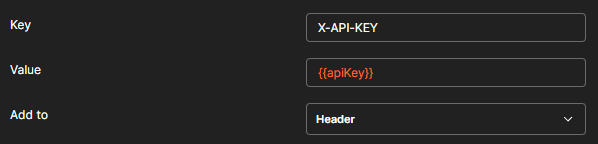
\includegraphics[width=0.7\textwidth]{Graphics/postmanauthscreen.png}
    \caption{Authentifizierung in Postman}
    \label{fig:authorization-postman}
\end{figure}

Zum Testen der Anfrage wird im \textit{Post-Request} Skript ein Testfall erstellt, welcher die Antwort auf den Statuscode 200 OK überprüft. Außerdem wird bestätigt, 
dass der Inhalt des Kommentars aktualisiert wurde (Listing~\ref{lst:post-request-script-200}). 

\begin{lstlisting}[language=JavaScript, caption=\textit{Post-Request} Skript für die Bearbeitung eines Kommentars,label=lst:post-request-script-200]
pm.test("Status code is 200", function () {
    pm.response.to.have.status(200);
});

// Test to check if the response contains updated comment data
pm.test("Response contains updated comment data", function () {
    var jsonData = pm.response.json();
    pm.expect(jsonData).to.have.property("id", parseInt(pm.collectionVariables.get("commentId")));
    pm.expect(jsonData).to.have.property("content", pm.collectionVariables.get("updatedCommentContent"));
    pm.expect(jsonData).to.have.property("authorId", parseInt(pm.collectionVariables.get("userId")));
    pm.expect(jsonData).to.have.property("postId", parseInt(pm.collectionVariables.get("postId")));
});
\end{lstlisting}

\subsubsection*{401 Unauthorized}

Um den Statuscode 401 Unauthorized zu testen, wird die Anfrage mit dem falschen \textit{\ac{API}-Key} gesendet. Zum Schluss muss dann nur der Statuscode getestet werden (Listing~\ref{lst:post-request-script-401}).

\begin{lstlisting}[language=JavaScript, caption=\textit{Post-Request} Skript für 401 Unauthorized,label=lst:post-request-script-401]
pm.test("Status code is 401", function () {
    pm.response.to.have.status(401);
});
\end{lstlisting}

\subsubsection*{404 Not Found}

Um den Statuscode 404 Not Found zu testen, wird die Anfrage einmal mit ungültiger Post-ID und einmal mit ungültiger Kommentar-ID gesendet. 
Die Tests sind identisch zu denen für 401 Unauthorized, nur dass der Statuscode 404 getestet wird (Listing~\ref{lst:post-request-script-404}).

\begin{lstlisting}[language=JavaScript, caption=\textit{Post-Request} Skript für 404 Not Found,label=lst:post-request-script-404]
pm.test("Status code is 404", function () {
    pm.response.to.have.status(404);
});
\end{lstlisting}

\subsection{Scenario Testing}

Beim \textit{Scenario Testing} werden mehrere Endpunkte in einer Sequenz getestet, um die Funktionalität der \ac{API} in verschiedenen Anwendungsfällen zu überprüfen. 
Dies ist oft bei komplexeren Anwendungsfällen nützlich, bei denen mehrere Endpunkte zusammenarbeiten müssen, um das gewünschte Ergebnis zu erzielen. 
So können besonders kritische Pfade in der \ac{API} getestet werden, um sicherzustellen, dass sie korrekt funktionieren. 
Dies ist vor allem notwendig bei Anwendungen, die auf einer umfangricheren \ac{API} basieren, wie z.B. Webanwendungen oder mobile Apps.
Ein Beispiel für ein simples Szenario wäre das ``Erstellen und Abrufen eines Posts'':

\begin{enumerate}
    \item \textbf{Ein Nutzer erstellt einen Post} - \textbf{POST /posts}
        \begin{itemize}
            \item existiert der Nutzer?
            \item sind alle Parameter vorhanden?
            \item ist der Inhalt des Posts valide?
            \item wird der Post erstellt?
        \end{itemize}
    \item \textbf{Der erstellte Post wird abgerufen} - \textbf{GET /posts/{{postId}}}
        \begin{itemize}
            \item existiert der Post?
            \item ist der Inhalt des Posts korrekt?
        \end{itemize}
    \item \textbf{Der erstellte Post wird gelöscht} - \textbf{DELETE /posts/{{postId}}}
        \begin{itemize}
            \item wird der Post gelöscht?
        \end{itemize}
\end{enumerate}

Da die \ac{API} in diesem Projekt relativ einfach ist, wurden keine komplexen Szenarien getestet, sondern nur die einzelnen Endpunkte.

\subsection{Automatisierung und Variablen}

Um eine effiziente Testausführung zu gewährleisten, wurden in Postman Variablen verwendet, 
um Werte wie \textit{postId} und \textit{authorId} zwischen den Testläufen dynamisch zu speichern. 
Dies ermöglichte eine Automatisierung der Testsequenzen, bei denen Ergebnisse aus einem Testlauf in den nächsten übernommen wurden. 
Zudem konnten Fehler bei ungültigen Eingaben erkannt werden, z.B. bei fehlenden Parametern oder unzulässigen Datentypen.
Die Verwendung von Postman ermöglichte die Durchführung dieser Tests sowohl manuell als auch automatisiert,
wobei alle Testfälle erfolgreich durchlaufen wurden und die Funktionalität der \ac{API} bestätigten.
Für die automatisierte Ausführung der Tests wurde eine \textit{\ac{CI}} Pipeline in Github Actions erstellt, welche bei jedem Push ausgeführt wird (siehe Continous Integration~\ref{sec:CI})./

\subsection{Bewertung}

Postman erweist sich als ein benutzerfreundliches und leistungsstarkes Werkzeug für API-Tests. 
Es bietet eine Vielzahl von Funktionen, die die Erstellung, Ausführung und Automatisierung von Tests erleichtern. 
Besonders hervorzuheben ist die Möglichkeit, Variablen zu verwenden, 
um Werte wie \textit{postId} und \textit{authorId} zwischen den Testläufen dynamisch zu speichern.
Außerdem ist die Vielseitigkeit von \textit{Collections} zur Strukturierung und Organisation von Testfällen sehr nützlich.
Dies ermöglicht eine effiziente und automatisierte Testausführung. 
Zudem können Fehler bei ungültigen Eingaben, wie fehlenden Parametern oder unzulässigen Datentypen, leicht erkannt werden.

Allerdings bringt das Always-Online-Modell von Postman auch einige Nachteile mit sich. 
Die ständige Abhängigkeit von der Postman API kann störend sein, insbesondere bei der Integrierung in \ac{CI}-Pipelines.
Zudem schränkt das Bezahlmodell die Anzahl der täglichen Testausführungen in der kostenlosen Version ein, 
was bei umfangreicheren Projekten zu erheblichen Einschränkungen führen kann.

Angesichts dieser Einschränkungen wäre es sinnvoll, für zukünftige Entwicklungen auch alternative Tools in Betracht zu ziehen. 
Tools wie \textit{Newman}, die CLI-Version von Postman, welche in der \ac{CI} Pipeline des Projekts verwendet wurde,
war hier eine nötige Ergänzung.

Andere API-Testwerkzeuge wie \textit{Hoppscotch}, \textit{Bruno}, \textit{Insomnia}, oder \textit{Katalon Studio} könnten eine gute Alternative darstellen, 
um die Abhängigkeit von der Postman Struktur zu reduzieren und die Flexibilität bei der Testausführung zu erhöhen.

Insgesamt bietet Postman eine solide Grundlage für API-Tests, 
jedoch sollten die genannten Einschränkungen bei der Planung und Durchführung von Tests berücksichtigt werden.
